% Part I: Aula 1 --- Does Organization Matter? Ford x GM x Toyota.
% Converted from Aula/aula-01-notes.md. Numbers checked against the md's formulas in Python
% (n_s = 1.5625, valley 83.926 at n_s; A = 30: 105.917 and 88.389; cube corners and orders).

\textbf{Syllabus item.} \emph{Aplicação: As organizações importam? Ford x GM x Toyota} (Topic 1).
\textbf{Read.} Milgrom \& Roberts (1992), Ch.~1 ``Does Organization Matter?'' (pp.~2--18);
Ch.~4 ``Coordination and Business Strategy'' (pp.~106--113); Cabral (2017) \S3.5 ``Why are firms
different?'' (pp.~56--59).

Page numbers are \MR's printed pages unless another book is named. Facts that do not come from
\MR\ carry their source inline; the stylized numbers are illustrative and checked by
\texttt{aula-01-companions/check\_companions.py} and the video's \texttt{check\_numbers.py}.
Three interactive companions in \texttt{Aula/aula-01-companions/} illustrate the formal part:
\texttt{two\_systems.html}, \texttt{valley.html} and \texttt{multiplier.html}.

% ---------------------------------------------------------------------------------------------
\section{The question}\label{sec:a1-question}

Ford had the technology, the scale and the cost advantage. GM beat it. Toyota was small, short of
capital and technologically behind. It beat GM. \MR's answer, which this class builds up to:

\begin{quote}
``organization and business strategy can be as important as technology, cost, and demand in
determining a firm's success'' \pg{16} --- and what matters most is ``the match of their
strategies and their structures'' \pg{16}.
\end{quote}

The class has two halves. First the cases, read as answers to two problems every organization
faces, \textbf{coordination} and \textbf{motivation} \pg{17}. Then the mathematics of
\textbf{fit}: complementarities, why they make good systems coherent, and why coherent systems are
hard to change one piece at a time.

% ---------------------------------------------------------------------------------------------
\section{Ford: one product, one system}\label{sec:a1-ford}

\MR's picture of Ford is short and exact: ``producing a single product (the Model T Ford) in
high-volume factories using specialized equipment and rigidly disciplined labor paid according to
the job being done'' \pg{109}. It was ``an entirely different but equally coherent strategy that
was appropriate for its time'' and it took Ford past 50\% of the US car market \pg{109}. By 1921
the Model T held \textbf{55\%} of the market, against \textbf{4\%} for Chevrolet and \textbf{11\%}
for all GM brands together \pg{2}.

The pieces, and why each raised the value of the others:

\begin{center}
\small
\begin{tabularx}{\linewidth}{@{}>{\raggedright\arraybackslash}p{0.27\linewidth}
  >{\raggedright\arraybackslash}X >{\raggedright\arraybackslash}X@{}}
\toprule
Choice & What it did & What it needed from the rest \\
\midrule
One model, one colour & long, identical runs & a buyer who wanted a cheap standard car \\
Dedicated machines, moving line & labour per car collapsed & huge, steady volume \\
Narrow, repetitive tasks & unskilled labour could be used & close supervision, a pay premium to
  keep workers \\
High wage (the $\$5$ day, 1914) & turnover fell & the productivity of the line to pay for it \\
Making its own parts & scale in components & the single design \\
\bottomrule
\end{tabularx}
\end{center}

History outside \MR\ (sources in
\texttt{Videos/\allowbreak aula-01-does-organization-matter/\allowbreak provenance.md}): the Model T sold for about
$\$850$ in 1908 and about $\$260$ by the mid-1920s; the moving chassis line (1913) cut assembly
time from about 12.5 hours to 93 minutes by early 1914; 1913 labour turnover was 370\% before the
$\$5$ day (Raff \& Summers 1987; the turnover figures are marked \emph{to confirm} there). The wage
story is efficiency wages, \MR\ Ch.~8 \pg{250}, outside this course's core.

\textbf{The weakness was the same as the strength.} Ford's 1920 answer to the recession was a price
cut of about 25\%, which GM, with higher costs, could not match \pg{2}. Cost leadership worked
while buyers wanted the same car. It stopped working when they wanted different cars.

% ---------------------------------------------------------------------------------------------
\section{GM: variety, and the organization it demanded}\label{sec:a1-gm}

Sloan took over a GM in crisis in 1921: unsold inventories piling up, sales down 75\% between
summer and fall 1920, divisions ``competed mostly with one another'' (pp.~2--3).

\textbf{Strategy.} A car ``for different segments of the market'': Cadillac at the top, each
division a lower-income segment, Chevrolet below the Model T's price \pg{3}.

\textbf{Why the strategy required a new organization.} Variety multiplied the decisions: new
designs, dealers, market information per segment, separate factories and supplies. At the same time
the divisions had to be coordinated: not compete too much, share ideas, coordinate R\&D,
standardize parts ``enough to achieve economies of scale in parts production'' \pg{3}. Neither
Ford's centralized one-product organization nor the old GM, ``a collection of car companies and
suppliers operating without any central direction'', could do this \pg{3}. The old accounting
system had not even charged divisions for the inventories they built up, so they kept producing
into the recession \pg{3}.

\textbf{The multidivisional form} \pg{3}:
\begin{itemize}
  \item divisions keep operating autonomy, each with its own management team and market segment;
  \item a strong central office does \emph{not} run day-to-day operations; it audits and evaluates
    divisions, plans and coordinates strategy, and keeps research, legal and financial functions;
  \item the centre checks internal accounting prices against market prices, so supply divisions
    can be judged ``as if each were a separate firm'' \pg{4}.
\end{itemize}

Henry Ford mocked the ``great big chart'' where a message takes six weeks to travel \pg{4}. The
result: from 1927 to 1937 Ford lost $\$200$ million and GM earned over $\$2$ billion; by 1940 GM
had 45\% of the market, Ford 16\% \pg{4}.

\textbf{GM's system fit together too.} Shared components across models let GM afford specialized
equipment for chassis, engines and brakes \pg{5}; its volumes fully used efficient parts plants, so
it integrated vertically \pg{5}, and it made suppliers compete on price \pg{6}. The price of
specialization: major redesigns only about every 12 years in the 1950s and 1960s \pg{5}.

% ---------------------------------------------------------------------------------------------
\section{Toyota: small, poor, and coherent in the other direction}\label{sec:a1-toyota}

Early-1950s Toyota had a ``drastic lack of capital'' and a scale too small to match US costs
\pg{4}. It first tried to copy mass production, then built a different system under Eiji Toyoda and
Taiichi Ohno \pg{4}.

\begin{center}
\small
\begin{tabularx}{\linewidth}{@{}>{\raggedright\arraybackslash}p{0.27\linewidth}
  >{\raggedright\arraybackslash}X >{\raggedright\arraybackslash}X@{}}
\toprule
Practice (\MR\ pp.~4--6) & Why it followed from Toyota's position & What it then required \\
\midrule
\textbf{Just-in-time / kanban}: no buffer inventories & inventory systems have large scale
  economies Toyota could not reach & every step reliable; defects caught at once \\
\textbf{Operators maintain and repair their own machines} & without buffers, a breakdown stops
  everything & broader skills, authority on the floor \\
\textbf{Flexible equipment}, quick resets, robots by the 1960s & too small to dedicate machines to
  one model & frequent model changes became cheap: redesign twice as often as GM \\
\textbf{Outside suppliers for complex components} & could neither reach efficient scale in parts
  nor afford to own parts makers & close day-to-day coordination with suppliers \\
\textbf{Few suppliers, long-term relations} & high-level components that must fit, frequent
  redesigns & suppliers willing to invest in Toyota-specific skills and machines \\
\bottomrule
\end{tabularx}
\end{center}

\MR's summary of the logic: ``If low inventories were to be achieved, the rest of the organization
had to emphasize reliability, quick response to machine breakdowns, quick and close communications
with suppliers, stable production plans, and other features that substitute for the buffer function
of inventories'' \pg{17}. Cabral adds why the system was hard to copy: ``the system involved so
many different aspects that it was difficult to pin down what the crucial success factors were''
(Cabral 2017, \S3.5, p.~57).

\subsection{Ford, GM, Toyota side by side}

\begin{center}
\small
\begin{tabularx}{\linewidth}{@{}>{\raggedright\arraybackslash}p{0.15\linewidth}
  >{\raggedright\arraybackslash}X >{\raggedright\arraybackslash}X
  >{\raggedright\arraybackslash}X@{}}
\toprule
Dimension & Ford (1910s) & GM (1920s on) & Toyota (1950s on) \\
\midrule
Product line & one model & a ladder of segments & several models, frequent redesign \\
Equipment & dedicated & specialized, shared components & flexible \\
Inventories & buffers & buffers & none (just-in-time) \\
Suppliers & made its own parts & vertically integrated; price competition & few, long-term,
  outside \\
Decisions & centralized in Henry Ford & divisions operate; centre audits and sets strategy &
  problem solving on the floor \\
Workers & narrow tasks, high wage & (not developed in \MR) & multi-skilled, maintain machines \\
\bottomrule
\end{tabularx}
\end{center}

\begin{keyidea}
Each column is coherent. None is a list of independent ``best practices''.
\end{keyidea}

% ---------------------------------------------------------------------------------------------
\section{Three more cases, one lesson each}\label{sec:a1-cases}

\MR\ widen the claim beyond cars (pp.~6--16). Each case isolates one piece of the argument.

\begin{itemize}
  \item \textbf{Hudson's Bay vs.\ North West Company} (pp.~6--9): \textbf{incentives and decision
    rights.} HBC had half the import costs, a royal monopoly and posts on the bay. It was run from
    London, with 15-month communication lags, flat salaries and rules enforced by flogging. NWC
    traders paddled an extra 1,500 miles. Its ``wintering partners'' decided on the spot and
    shared the profits. By about 1810 NWC had nearly 80\% of the trade \pg{8}. HBC recovered only
    by copying the \emph{organization}: inland posts, half of profits to field officers, more
    freedom of action (pp.~8--9).
  \item \textbf{Salomon Brothers} (pp.~9--12): \textbf{incentives that are too individual.} Near
    piece-rate bonuses made traders work hard and take risks but discouraged sharing information
    across departments \pg{11}. The 1990 reform paid part of each bonus in stock held in trust for
    five years; the announcement raised the firm's value by 7--10\% \pg{12}. FFT~1.3 \pg{18} asks
    what the 1991 scandal says about that scheme.
  \item \textbf{Eastern Europe} (pp.~12--16): \textbf{information, incentives and interdependent
    reforms.} Central planning replaced prices with vertical information flows \pg{13}. The
    \textbf{ratchet effect}: a manager who beats the quota gets a higher quota, so nobody beats it;
    capacity is hidden and resources hoarded \pg{14}. Reform pieces depend on each other (property
    rights, capital markets, contract enforcement), so ``the worst outcome might be some halfway
    compromise'' \pg{16}: the country that moved only its trucks to the other side of the road.
    The ratchet effect returns in Aula 16 (\MR\ p.~232).
\end{itemize}

% ---------------------------------------------------------------------------------------------
\section{The patterns: coordination, motivation, and fit (pp.~16--17)}\label{sec:a1-patterns}

\MR\ draw four patterns out of the cases.

\begin{enumerate}
  \item \textbf{Organization and strategy can matter as much as technology, cost and demand.} Ford
    lost to GM despite better technology and scale; GM lost share to a smaller, weaker Toyota; HBC
    lost to NWC \pg{16}.
  \item \textbf{Incentives matter.} HBC employees got no share of extra profits; GM's divisions
    were not charged for inventories; Salomon rewarded individuals and so discouraged cooperation;
    planned economies ``ran afoul of incentives at every turn'' \pg{16}.
  \item \textbf{Put authority where the information is.} Salomon's traders, GM's divisions,
    Toyota's operators, NWC's wintering partners \pg{17}.
  \item \textbf{Incentives and delegated authority are complements.} Delegation is worth little
    ``unless the decision makers share the organization's objectives'', and incentives matter most
    ``when more initiative is expected from employees''. In \MR's words: ``incentives and delegated
    authority are complements: each makes the other more valuable'' \pg{17}.
\end{enumerate}

And the organizing pair for the course:

\begin{keyidea}
``The study of organization is not about how berries are arranged on a tree of authority but about
how people are coordinated and motivated to get things done'' \pg{16}.
\end{keyidea}

\begin{center}
\small
\begin{tabularx}{\linewidth}{@{}>{\raggedright\arraybackslash}p{0.14\linewidth}
  >{\raggedright\arraybackslash}X >{\raggedright\arraybackslash}X@{}}
\toprule
 & \textbf{Coordination}: getting the plans to fit (information) & \textbf{Motivation}: getting
   people to carry them out (interests) \\
\midrule
Ford & one product, one centre, the line sets the pace & high wage, close supervision \\
GM & divisions per segment; centre plans strategy, shared parts & divisions judged on profit,
  internal prices checked against the market \\
Toyota & just-in-time signals, close supplier links & multi-skilled teams, long-term supplier
  relations \\
HBC $\to$ NWC & decisions moved to the field & profit shares for those deciding \\
\bottomrule
\end{tabularx}
\end{center}

Course map: coordination in Aulas 6--8 (\MR\ Ch.~3--4), motivation in Aulas 9--16 (Ch.~5--7).

% ---------------------------------------------------------------------------------------------
\section{Complementarities: the mathematics of fit (\MR\ Ch.~4, pp.~108--109)}
\label{sec:a1-compl}

\subsection{Definition}\label{sec:a1-def}

The market definition: two inputs are complements if a fall in the price of one raises demand for
the other. \MR\ use a ``more inclusive'' definition that also covers internal activities:

\begin{defn}{Complementary activities (\MR\ p.~108)}
``Several activities are mutually complementary if doing more of any one activity increases (or at
least does not decrease) the marginal profitability of each other activity in the group''
\pg{108}.

\textbf{Smooth version} (footnote 8, p.~108). With activity levels $x = (x_1, \dots, x_n)$ and
profit $\pi(x)$:
\[
  \frac{\partial^2 \pi}{\partial x_i \, \partial x_j} \;\ge\; 0 \qquad \text{for all } i \ne j .
\]

\textbf{Discrete version: increasing differences.} For two yes/no choices $x, y \in \{0, 1\}$:
\[
  \underbrace{\pi(1,1) - \pi(0,1)}_{\text{gain from } x \text{ when } y = 1} \;\ge\;
  \underbrace{\pi(1,0) - \pi(0,0)}_{\text{gain from } x \text{ when } y = 0}.
\]
\end{defn}

\begin{prop}{Result: increasing differences is symmetric and equals supermodularity}
Rearranging the same inequality three ways:
\begin{align*}
  \pi(1,1) - \pi(0,1) \ge \pi(1,0) - \pi(0,0)
  &\iff \pi(1,1) + \pi(0,0) \ge \pi(1,0) + \pi(0,1) \\
  &\iff \pi(1,1) - \pi(1,0) \ge \pi(0,1) - \pi(0,0).
\end{align*}
The last line says the gain from $y$ is larger when $x = 1$ (symmetry). The middle line is
\textbf{supermodularity}: the two ``matched'' corners together beat the two ``mixed'' ones.
\end{prop}

\begin{example}{The video's $2\times 2$ table}
$\pi(0,0)=0$, $\pi(1,0)=-2$, $\pi(0,1)=-1$, $\pi(1,1)=5$.
\begin{itemize}
  \item Gain from $x$ when $y=0$: $-2 - 0 = -2$; when $y = 1$: $5 - (-1) = 6$. Increasing
    differences hold.
  \item Each practice \textbf{alone loses money}, and the pair gains 5. The cross effect is
    $6 - (-2) = 8$.
  \item A firm that tests each practice separately rejects both.
\end{itemize}
\end{example}

\begin{keyidea}
Complementarity says nothing about whether each practice is good on its own. It says each is
\textbf{better where the other is present}.
\end{keyidea}

\subsection{Why complements move together}\label{sec:a1-move}

\textbf{One choice, one parameter (Topkis, stated).} If $x^*(t)$ maximizes $f(x, t)$ and $f$ is
concave in $x$, differentiate the first-order condition $f_x(x^*(t), t) = 0$ with respect to $t$:
\[
  f_{xx}\, x^{*\prime}(t) + f_{xt} = 0 \;\;\Longrightarrow\;\;
  x^{*\prime}(t) = -\frac{f_{xt}}{f_{xx}} \;\ge\; 0 \quad\text{whenever } f_{xt} \ge 0 ,
\]
since concavity gives $f_{xx} < 0$ at an interior optimum where the implicit function theorem
applies.

\begin{prop}{Theorem (Topkis)}
If $f$ has increasing differences in $(x, t)$, the optimal $x$ is non-decreasing in $t$. No
derivatives or concavity are needed.
\end{prop}

Milgrom \& Roberts (1990, \emph{AER} 80(3), 511--528) used it to explain why the elements of modern
manufacturing were adopted together. Stated, not proved: the lattice proof is beyond the course.

\textbf{Two choices, the systems effect.} Let $x$ be delegated authority and $y$ incentive
intensity (\MR's p.~17 pair), with
\[
  \pi(x, y) = t x + s y + b\, x y - \tfrac{c}{2} x^2 - \tfrac{c}{2} y^2, \qquad
  \frac{\partial^2 \pi}{\partial x\, \partial y} = b .
\]
First-order conditions:
\[
  \pi_x = t + b y - c x = 0, \qquad \pi_y = s + b x - c y = 0
  \quad\Longleftrightarrow\quad t + b y = c x, \qquad s + b x = c y .
\]
From the first, $x = (t + b y)/c$. Substituting into the second, $s + b(t + by)/c = cy$, i.e.\
$cs + bt + b^2 y = c^2 y$, so $y^* = (cs + bt)/(c^2 - b^2)$; by symmetry of the two conditions,
\[
  x^* = \frac{c t + b s}{c^2 - b^2}, \qquad y^* = \frac{c s + b t}{c^2 - b^2}, \qquad
  \text{a maximum iff } c > |b| .
\]
The Hessian is $\begin{psmallmatrix} -c & b \\ b & -c \end{psmallmatrix}$: negative definite iff
$-c < 0$ and $c^2 - b^2 > 0$, which together are $c > |b|$.

How delegation responds to more valuable local information $t$:
\[
  \frac{\partial x^*}{\partial t} = \frac{c}{c^2 - b^2} = \frac{1}{c} \cdot \frac{1}{1 - (b/c)^2}
  = \frac{1}{c}\Big(1 + \big(\tfrac{b}{c}\big)^2 + \big(\tfrac{b}{c}\big)^4 + \cdots\Big), \qquad
  \frac{\partial y^*}{\partial t} = \frac{b}{c^2 - b^2}.
\]

\begin{itemize}
  \item $1/c$ is the response with $y$ held fixed. The geometric series is \MR's footnote 8 in
    numbers: more $x$ raises the return to $y$, more $y$ raises the return to $x$, ``possibly
    leading to another round of increases'' \pg{108}.
  \item $t$ never enters the condition for $y$, yet $y^*$ moves: with $b > 0$ incentives rise when
    delegation becomes more valuable.
  \item At $c = 2$, $b = 1$: multiplier $1/(1 - 1/4) = 4/3$. With $t$ from 1 to 3 ($s = 1$), $x^*$
    goes from 1 to $7/3$ instead of from $0.5$ to $1.5$.
  \item With \textbf{substitutes} ($b < 0$) the multiplier is still above one, because
    $(b/c)^2 > 0$: incentives fall, which raises delegation's return again. Only the sign of
    $\partial y^*/\partial t$ flips.
\end{itemize}

\begin{keyidea}
The companion \texttt{multiplier.html} (The Complementarity Multiplier) illustrates this: moving $t$
shows the staircase of rounds, $b = 0$ makes the multiplier fall to 1, and pushing $|b|$ toward $c$
makes it explode until the optimum vanishes.
\end{keyidea}

\subsection{Substitutes are complements upside down}\label{sec:a1-subs}

If $\partial^2 f/\partial x\,\partial y \le 0$ (buffer inventories and floor-level problem solving
are substitutes: each makes the other less needed), define $z = -y$ and $g(x, z) = f(x, -z)$. Then
$g_{xz} = -f_{xy} \ge 0$. Every result above applies to $(x, z)$. ``Many buffers, narrow jobs''
(Ford) and ``no buffers, problem solvers'' (Toyota) are both coherent; the mixtures are not.

\subsection{Strong complementarity and design attributes \pg{109}}\label{sec:a1-strong}

Complementarity makes the choices \textbf{predictable}: high levels go together. \MR\ add a
second, separate feature, the \textbf{high cost of failing to fit}, and call a group
\emph{strongly complementary} when raising some activities ``greatly increases the returns'' to
raising the others; then ``design attributes are always present'' \pg{109}. The box ``Modern
Manufacturing Strategy'' (pp.~109--110) traces one chain:
\begin{quote}
small demand per product $\to$ no finished-goods inventories $\to$ close sales--factory
communication $\to$ short production runs $\to$ frequent changeovers $\to$ flexible equipment
$\to$ multi-skilled workers paid for skills, not piece rates $\to$ machine-time cost accounting.
\end{quote}

% ---------------------------------------------------------------------------------------------
\section{More than one coherent system (\MR\ Ch.~4, pp.~111--113)}\label{sec:a1-systems}

\subsection{Figure 4.3, made exact}\label{sec:a1-fig43}

\MR's figure: a \textbf{marketing manager} chooses the number of product varieties $n$; a
\textbf{manufacturing manager} chooses the batch size $b$ \pg{111}. More varieties at a fixed batch
size raise inventories, so the larger the batch, the fewer varieties are worth offering; more
varieties raise the marginal inventory cost of a larger batch, so the more varieties, the smaller
the best batch \pg{111}. Both best replies slope down, and they can cross more than once \pg{112}.

\MR\ draw the curves without a formula. A form that produces them, with equipment
$\theta \in \{\text{specialized}, \text{flexible}\}$ added (pp.~5, 113):
\[
  \pi(n, b, \theta) = mQ + A \ln n - \frac{S_\theta Q}{b} - \frac{h\, n\, b}{2}
  - \Delta c_\theta\, Q, \qquad n \ge 1,
\]
where $A$ is the taste for variety, $Q$ total volume, $S_\theta Q / b$ the changeover cost ($Q/b$
changeovers), $h n b / 2$ the cost of holding average inventory $b/2$ for each of $n$ models, and
$\Delta c_\theta$ the unit-cost premium of flexible equipment (zero for specialized).

\begin{itemize}
  \item \textbf{Manufacturing's reply (the EOQ formula).} $\pi_b = S_\theta Q/b^2 - hn/2 = 0$
    gives $b^*(n) = \sqrt{2 S_\theta Q / (h n)}$, decreasing in $n$.
  \item \textbf{Marketing's reply.} $\pi_n = A/n - hb/2 = 0$, so
    $A/n = h b / 2 \Rightarrow n^*(b) = \max\{1, \; 2A/(h b)\}$, decreasing in $b$.
  \item \textbf{Cross effect.} $\partial^2 \pi / \partial n\, \partial b = -h/2 < 0$: variety and
    batch size are substitutes, so variety and \textbf{small batches} are complements
    (\S\ref{sec:a1-subs}).
  \item \textbf{Within one equipment type.} Substituting $n = 2A/(hb)$ into $S Q/b^2 = hn/2$ gives
    $SQ/b^2 = A/b$, so $b^* = S Q / A$ and $n^* = 2A^2/(h S Q)$. At the optimum
    $SQ/b^* = A$ and $hn^*b^*/2 = A$, so $\pi^* = mQ + A \ln n^* - 2A - \Delta c\, Q$. Corner
    $n^* = 1$ (Ford's single model) when $2A^2 \le h S Q$.
  \item \textbf{The equipment switch.} At the EOQ batch the two batch-related costs are equal, so
    $S Q/b^* + h n b^*/2 = \sqrt{2 S Q h n}$. Flexible equipment is cheaper once
    $\sqrt{2Qhn}\,(\sqrt{S_s} - \sqrt{S_F}) \ge \Delta c\, Q$, i.e.\ once $n$ exceeds
    \[
      n_s = \frac{(\Delta c\, Q)^2}{2 Q h \big(\sqrt{S_s} - \sqrt{S_F}\big)^2}.
    \]
    Manufacturing's reply \textbf{jumps down} there.
\end{itemize}

With the companion's calibration ($A = 20$, $Q = 100$, $h = 1$, $S_s = 50$, $S_F = 2$,
$\Delta c = 1$, $m = 2$):

\begin{center}
\begin{tabular}{@{}lccc@{}}
\toprule
System & $n^*$ & $b^*$ & Profit \\
\midrule
Specialized (Ford-type) & 1 (corner) & 100 & 100.0 \\
Flexible (Toyota-type) & 4 & 10 & 87.7 \\
\bottomrule
\end{tabular}
\end{center}

Here $\sqrt{S_s} - \sqrt{S_F} = 5\sqrt2 - \sqrt2 = 4\sqrt2$, so
$n_s = 100^2/(2\cdot 100\cdot 32) = 1.5625$. Manufacturing's reply is $b = 100/\sqrt{n}$ for
$n \le n_s$ and $b = 20/\sqrt{n}$ beyond it, dropping from 80 to 16 at $n_s$. Marketing's reply is
$n = 1$ for $b \ge 40$ and $n = 40/b$ below.

Both are coherent: at each, neither manager wants to move. Between them, profit along
manufacturing's reply falls to \textbf{83.9}. Raise $A$ to 30 and the flexible system earns 105.9,
better than 100, yet the valley is still there (88.4).

\begin{figure}[ht]
\centering
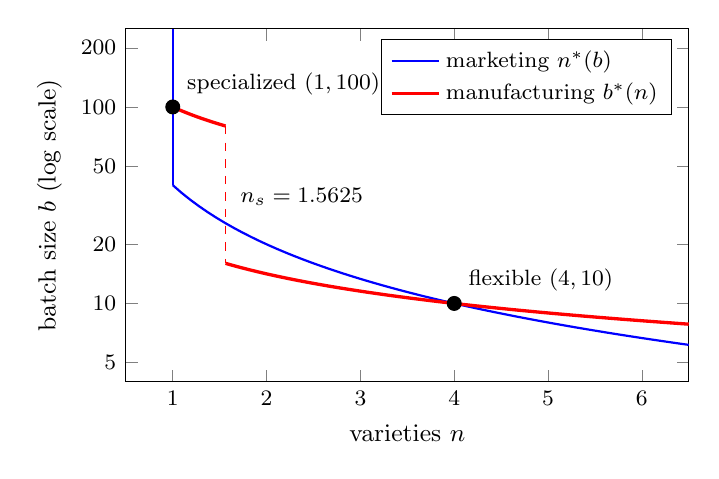
\begin{tikzpicture}
\begin{axis}[
  width=0.72\linewidth, height=0.5\linewidth,
  xmin=0.5, xmax=6.5, ymin=4, ymax=250, ymode=log,
  xlabel={varieties $n$}, ylabel={batch size $b$ (log scale)},
  ytick={5,10,20,50,100,200}, yticklabels={5,10,20,50,100,200},
  xtick={1,2,3,4,5,6},
  legend pos=north east, legend style={font=\footnotesize, cells={anchor=west}},
  tick label style={font=\footnotesize}, label style={font=\small},
  clip=false]
  % marketing: n = max{1, 40/b}
  \addplot[thick, blue, domain=1:6.5, samples=60] {40/x};
  \addlegendentry{marketing $n^*(b)$}
  \addplot[very thick, red, domain=1:1.5625, samples=20] {100/sqrt(x)};
  \addlegendentry{manufacturing $b^*(n)$}
  \addplot[thick, blue, forget plot] coordinates {(1,40) (1,250)};
  \addplot[very thick, red, domain=1.5625:6.5, samples=60, forget plot] {20/sqrt(x)};
  \addplot[red, dashed, forget plot] coordinates {(1.5625,80) (1.5625,16)};
  \node[font=\footnotesize, anchor=west] at (axis cs:1.62,35) {$n_s = 1.5625$};
  \addplot[only marks, mark=*, mark size=2.5pt, black, forget plot]
    coordinates {(1,100) (4,10)};
  \node[font=\footnotesize, anchor=south west] at (axis cs:1.05,102) {specialized $(1,100)$};
  \node[font=\footnotesize, anchor=south west] at (axis cs:4.05,10.3) {flexible $(4,10)$};
\end{axis}
\end{tikzpicture}
\caption{Figure 4.3 made exact, with $A=20$, $Q=100$, $h=1$, $S_s=50$, $S_F=2$, $\Delta c=1$.
Marketing's reply is $n^*(b)=\max\{1,2A/(hb)\}$ (vertical at $n=1$ for $b\ge 40$); manufacturing's
reply $b^*(n)=\sqrt{2SQ/(hn)}$ jumps from 80 to 16 at $n_s=1.5625$, where it switches from
specialized to flexible equipment. The two crossings are the two coherent systems.}
\label{fig:a1-fig43}
\end{figure}

\subsection{What the figure teaches}\label{sec:a1-teaches}

\begin{itemize}
  \item \textbf{Alignment is not optimality.} Each crossing is ``a coherent strategy'' \pg{112};
    ``only one combination is actually profit maximizing'' \pg{112}. Ford's crossing was best for
    the early century; the many-varieties, small-batch crossing is best for many industries now
    \pg{112}.
  \item \textbf{Local adjustment cannot find the global shift.} Managers can track the
    \emph{local} movement of their own crossing, ``but recognizing that a radical strategic shift is
    desirable is likely to require information that neither manager has'' \pg{113}. Smooth changes
    in the curves can hide a jump in which crossing is best \pg{112}.
  \item \textbf{So the choice among coherent patterns is a job for central management} (p.~113,
    p.~115), with innovation attributes, because the information is outside the organization. This
    is Aula 7's argument, met here first.
\end{itemize}

\begin{caution}{A careful reading of footnote 9}
\MR\ picture the profit surface as ``a mountain with three peaks, one at each of the
intersections'' \pg{112}. With two \emph{smooth} decreasing best replies that cross three times,
the middle crossing is a \textbf{saddle}, not a peak: there the replies cross the ``wrong'' way,
$\pi_{nb}^2 > \pi_{nn}\pi_{bb}$, and the Hessian is indefinite. The outer two crossings are the
peaks. The book's point is unaffected: several coherent systems, one best.
\end{caution}

\begin{keyidea}
The companion \texttt{two\_systems.html} (Two Coherent Systems) illustrates this: its plate 1 is
Figure 4.3, its plate 2 the ``ridge line'' of footnote 9, and its presets \emph{More taste for
variety} and \emph{Cheaper flexibility} move each system a little while the best one switches.
\end{keyidea}

% ---------------------------------------------------------------------------------------------
\section{The valley, and the plant that tested it}\label{sec:a1-valley}

\subsection{Three practices on a cube}\label{sec:a1-cube}

Take three Toyota practices from \S\ref{sec:a1-toyota}: just-in-time $J$, multi-skilled teams $T$,
long-term suppliers $S$, each 0 or 1. The class's stylized payoff:
\[
  \pi(J, T, S) = 10 - 4J - 2T - S + 4JT + 5JS + 2TS + 2JTS .
\]

\begin{center}
\small
\setlength{\tabcolsep}{4pt}
\begin{tabular}{@{}lcccccccc@{}}
\toprule
Corner & 000 & 100 & 010 & 001 & 110 & 101 & 011 & 111 \\
\midrule
Profit & \textbf{10} (Ford) & 6 & 8 & 9 & 8 & 10 & 9 & \textbf{16} (Toyota) \\
\bottomrule
\end{tabular}
\end{center}

\begin{itemize}
  \item Supermodular: the pairwise gains $4 + 2S$, $5 + 2T$, $2 + 2J$ are all positive.
  \item \textbf{Every first step loses}: 6, 8, 9 $<$ 10. Ford's corner is a local peak.
  \item \textbf{Every adoption order dips.} Of the six orders from 000 to 111, the best one still
    falls to 9 before reaching 16.
  \item 111 is also a local peak (its neighbours earn 9, 10, 8). Two peaks, and marginal analysis
    cannot tell them apart: the package gain is $+6$; the best single step is $-1$.
\end{itemize}

\begin{figure}[ht]
\centering
\begin{tikzpicture}
\begin{axis}[
  width=0.68\linewidth, height=0.46\linewidth,
  xmin=-0.2, xmax=3.2, ymin=4, ymax=18,
  xtick={0,1,2,3}, xticklabels={000,1st step,2nd step,111},
  ytick={6,8,10,12,14,16},
  xlabel={practices adopted}, ylabel={profit $\pi(J,T,S)$},
  legend pos=north west, legend style={font=\footnotesize, cells={anchor=west}},
  tick label style={font=\footnotesize}, label style={font=\small}]
  \addplot[gray!60, mark=o, mark size=1.5pt] coordinates {(0,10) (1,6) (2,8) (3,16)};
  \addlegendentry{other orders}
  \addplot[gray!60, mark=o, mark size=1.5pt, forget plot] coordinates {(0,10) (1,6) (2,10) (3,16)};
  \addplot[gray!60, mark=o, mark size=1.5pt, forget plot] coordinates {(0,10) (1,8) (2,8) (3,16)};
  \addplot[gray!60, mark=o, mark size=1.5pt, forget plot] coordinates {(0,10) (1,8) (2,9) (3,16)};
  \addplot[orange, thick, mark=square*, mark size=1.5pt] coordinates {(0,10) (1,9) (2,9) (3,16)};
  \addlegendentry{order $S$, $T$, $J$}
  \addplot[exc, very thick, mark=*, mark size=2pt] coordinates {(0,10) (1,9) (2,10) (3,16)};
  \addlegendentry{order $S$, $J$, $T$}
  \addplot[black, dashed, domain=-0.2:3.2] {10};
  \addlegendentry{Ford level (10)}
\end{axis}
\end{tikzpicture}
\caption{Profit along the six adoption orders from 000 (Ford) to 111 (Toyota), read off the corner
table. Every order dips below the Ford level 10; the best orders, which adopt $S$ first, fall to 9
before reaching 16.}
\label{fig:a1-valley}
\end{figure}

\begin{keyidea}
Complementarity tells you \textbf{where} the optimum is (all practices together). It does not make
the road uphill. It \textbf{creates} the valley, because a practice is worth least where its
complements are missing.
\end{keyidea}

\begin{keyidea}
The companion \texttt{valley.html} (The Valley Between Systems) illustrates this: its preset
\emph{No interactions} shows ``best practices'' thinking (profits add up and the package loses),
and \emph{No stand-alone losses} lets some order climb without a dip.
\end{keyidea}

\subsection{NUMMI: the same workers under two systems}\label{sec:a1-nummi}

History outside \MR\ (sources and status in
\texttt{Videos/\allowbreak aula-01-does-organization-matter/\allowbreak provenance.md}):

\begin{itemize}
  \item GM closed its Fremont, California plant in 1982. It reopened in 1984 as \textbf{NUMMI}, a
    GM--Toyota joint venture run on Toyota's system, and over 85\% of its first workforce were the
    laid-off GM workers.
  \item 1987 assembly hours per car: \textbf{31} at a comparable GM plant (Framingham),
    \textbf{19} at NUMMI, 16 at Toyota's Takaoka plant; assembly defects per 100 cars 135, 45 and
    45. These figures come from a secondary reproduction of Womack, Jones \& Roos (1990) and are
    marked \emph{to confirm against the book}.
  \item GM owned half the plant and its managers could study it, yet its efforts to spread the
    system piece by piece across its US plants ``proved largely unsuccessful''. The exception was
    Brazil, where NUMMI-trained managers ran the transfer.
\end{itemize}

Read with \S\ref{sec:a1-cube}: Toyota moved the whole system at once (the jump across the valley).
GM, adopting practice by practice, kept landing on the low corners.

\subsection{Evidence beyond one plant}\label{sec:a1-evidence}

A test regression: $y = \beta_0 + \beta_1 x + \beta_2 z + \beta_3 x z + \varepsilon$. The effect of
$x$ is $\beta_1$ when $z = 0$ and $\beta_1 + \beta_3$ when $z = 1$: $\beta_3$ is the cross effect.
Ichniowski, Shaw \& Prennushi (1997, \emph{AER} 87(3), 291--313), on 36 steel finishing lines: the
bundle of innovative HR practices raises productivity; single practices adopted in isolation do
not.

\begin{caution}{Correlated adoption is not proof}
Firms that adopt practices together may differ in other ways, so correlated adoption alone does
not prove complementarity.
\end{caution}

% ---------------------------------------------------------------------------------------------
\section{Common mistakes}\label{sec:a1-mistakes}

\begin{center}
\small
\begin{tabularx}{\linewidth}{@{}>{\raggedright\arraybackslash}p{0.33\linewidth}
  >{\raggedright\arraybackslash}X@{}}
\toprule
Mistake & Correction \\
\midrule
``Copy best practices one at a time'' & Profit is not additive; with complements, a practice
  adopted alone can lose money (\S\ref{sec:a1-def}, \S\ref{sec:a1-cube}). \\
``Complements means each is good'' & Complements means each is \emph{better with} the other. Both
  can lose alone (the $2\times2$ table). \\
``A coherent system is the best system'' & Coherence is a local property. Several coherent
  systems coexist; only one is best (\S\ref{sec:a1-teaches}). \\
``If it is better, managers will drift to it'' & Marginal adjustment stays at a local peak;
  reaching the other needs a coordinated jump (pp.~112--113). \\
Using the market definition of complements (cross-price) for internal choices & \MR's definition
  is about marginal profitability, $\partial^2\pi/\partial x_i\partial x_j \ge 0$ \pg{108}. \\
``Substitutes have a multiplier below one'' & In the two-choice model the own response is
  amplified for either sign of $b$; only the other choice's direction changes
  (\S\ref{sec:a1-move}). \\
Reading organization as the org chart & ``not about how berries are arranged on a tree of
  authority but about how people are coordinated and motivated'' \pg{16}. \\
\bottomrule
\end{tabularx}
\end{center}

% ---------------------------------------------------------------------------------------------
\section{Exercises (number and page only)}\label{sec:a1-exercises}

\begin{center}
\small
\begin{tabularx}{\linewidth}{@{}>{\raggedright\arraybackslash}p{0.3\linewidth}
  l >{\raggedright\arraybackslash}X@{}}
\toprule
Exercise & Where & Practises \\
\midrule
\MR\ Food for Thought 1.1 & p.~18 & splitting a business's decisions between centre and units;
  coordination vs.\ motivation \\
\MR\ Food for Thought 1.2 & p.~18 & the same split in a non-business organization \\
\MR\ Food for Thought 1.3 & p.~18 & the Salomon incentive scheme (\S\ref{sec:a1-cases}) against a
  later scandal \\
Cabral 1.1 & p.~11 & competition and performance \\
Cabral 3.14 & p.~63 & sustained competitive advantage (\S3.5) \\
Cabral 3.20 & p.~64 & productivity dispersion across firms (applied, data) \\
\bottomrule
\end{tabularx}
\end{center}

For the formal part (\S\ref{sec:a1-compl}--\S\ref{sec:a1-valley}) there are no book exercises in
\MR\ Ch.~1; use the companions' presets as problems: predict the read-out, then move the control.

% ---------------------------------------------------------------------------------------------
\section*{Sources}
\addcontentsline{toc}{section}{Sources}

\begin{itemize}
  \item Milgrom, P.\ \& Roberts, J.\ (1992). \emph{Economics, Organization, and Management}.
    Prentice-Hall. Ch.~1 (pp.~2--18), Ch.~4 (pp.~106--115). Read from \texttt{Livros/} on
    2026-10-09.
  \item Milgrom, P.\ \& Roberts, J.\ (1990). ``The Economics of Modern Manufacturing: Technology,
    Strategy, and Organization''. \emph{American Economic Review} 80(3), 511--528.
  \item Cabral, L.\ (2017). \emph{Introduction to Industrial Organization}, 2nd ed. MIT Press.
    \S3.5, pp.~56--59.
  \item Ichniowski, C., Shaw, K.\ \& Prennushi, G.\ (1997). \emph{American Economic Review} 87(3),
    291--313.
  \item Ford and NUMMI history: \texttt{Videos/\allowbreak aula-01-does-organization-matter/\allowbreak provenance.md}
    (each claim with its source and status).
\end{itemize}
